\label{sec:method}
\section{Methodology}

\begin{figure}[tb]
  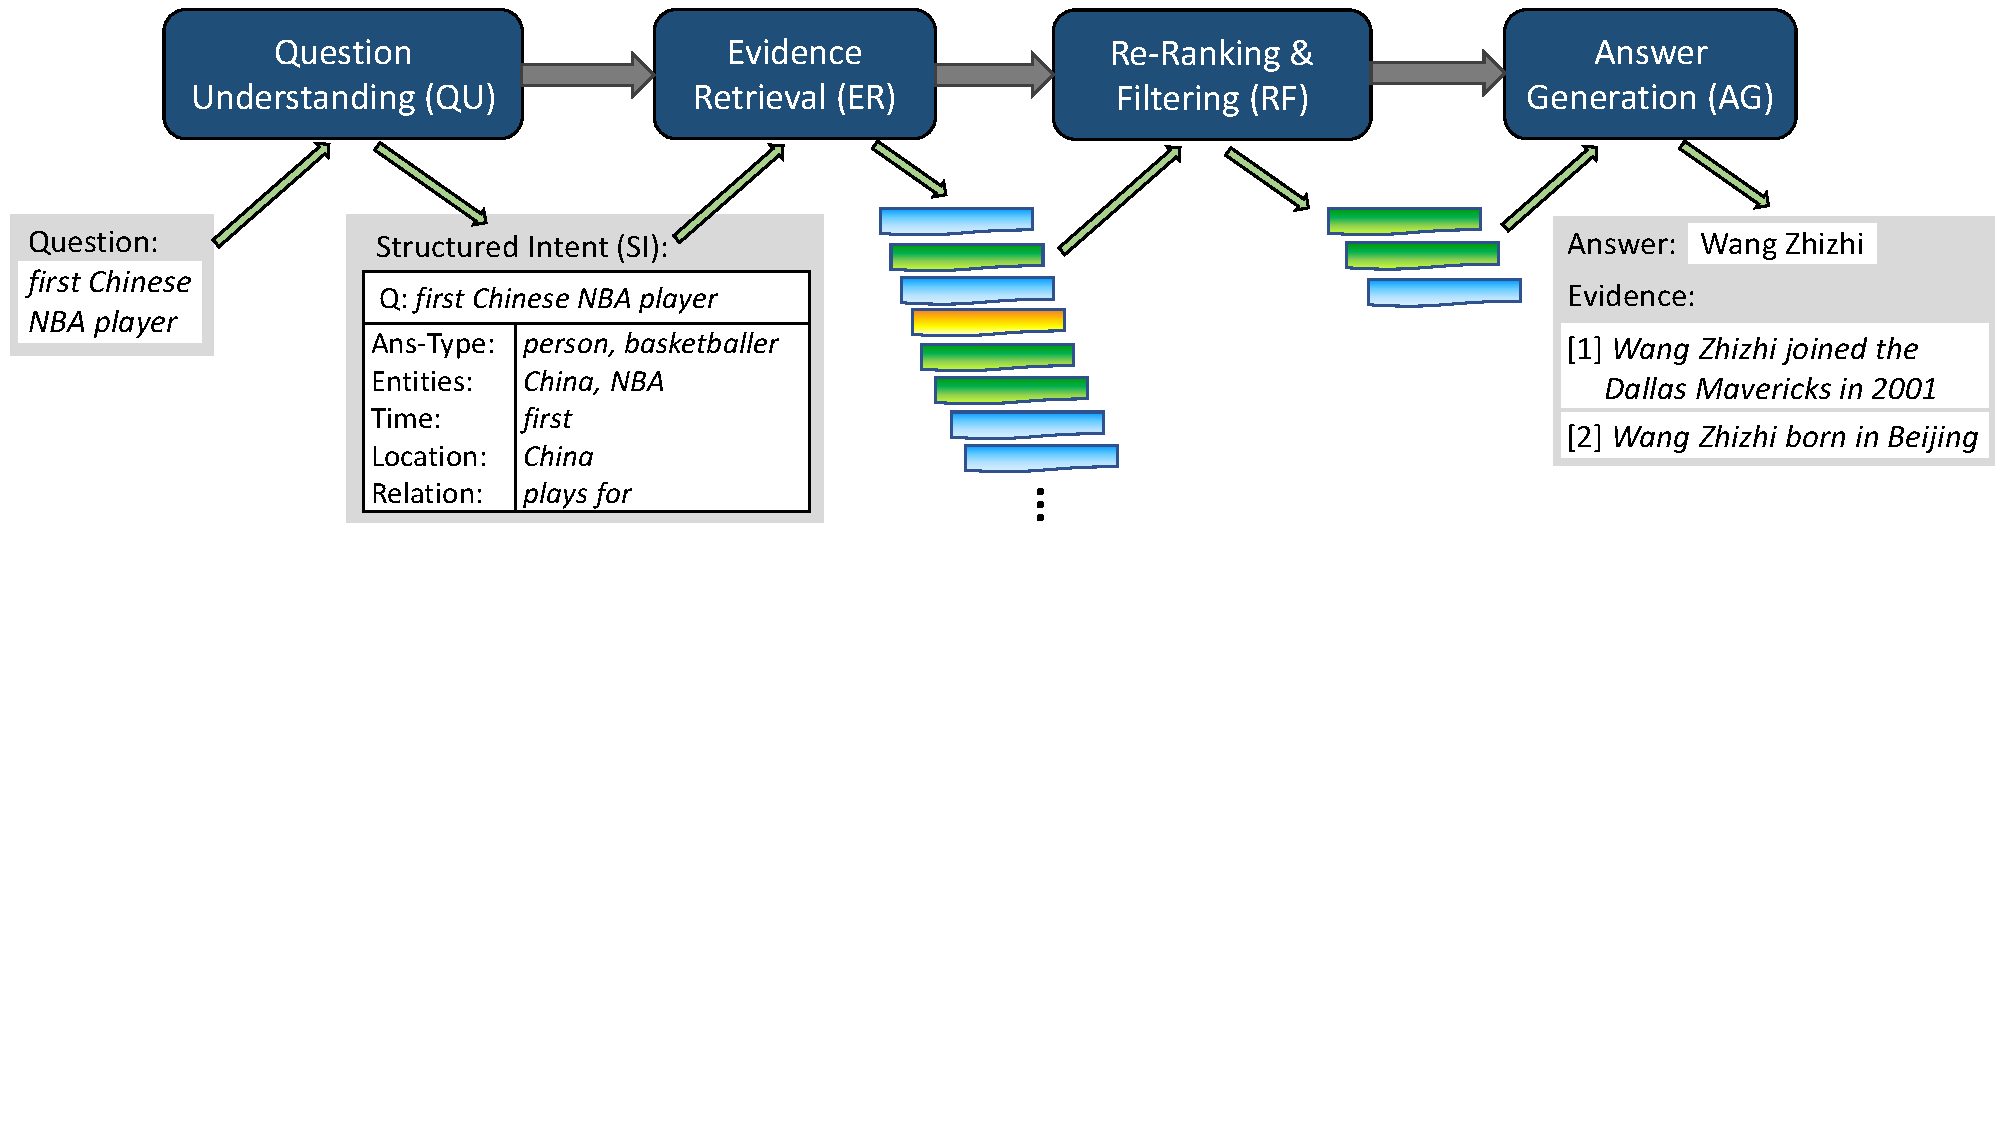
\includegraphics[width=\textwidth]{submissions/Gerhard2024/figures/compass-overview.pdf}
  \caption{Overview of the \method system.}
  \label{fig:compass-overview}
\end{figure}

% start with system overview
The \method system is a pipeline of four major stages, as illustrated in Figure \ref{fig:compass-overview}.
First, the input question is analyzed and decomposed, in order to compute a {\em structured intent (SI)} representation that will pass on to the subsequent steps, along with the original question. Second, the SI is utilized to retrieve pieces of evidence from different sources: text, KG and tables. 
Third, this pool of potentially useful evidence is filtered down, with iterative re-ranking, to arrive at a tractably small set of most promising evidence.
The final stage generates the answer from this evidence,
passing back the answer as well as evidence snippets for user-comprehensible explanation.

The second and fourth stage, Evidence Retrieval (ER) and Answer Generation (AG), are fairly standard. Such a two-phase architecture was called a retriever-reader architecture~\cite{Zhu-ODQA-survey:arxiv2021}. With a modern LLM replacing the earlier kinds of neural readers, this is the core of every RAG system~\cite{DBLP:journals/arXiv/abs-2312-10997}.

Stages 1 and 3 are unique elements of our architecture, judiciously introduced to improve both effectiveness (i.e., answer quality) and efficiency (i.e., computational cost).
Question Understanding (QU) provides the ER component with crisper and semantically refined input, and
the Re-Ranking \& Filtering (RF) stage is beneficial for
distilling the best evidence from the large pool of retrieved pieces.
The following subsections elaborate on the four stages of the pipeline, emphasizing the \method-specific steps QU and RF.



\subsection{Question Understanding (QU)}

% one par introducing the SI
To prepare the retrieval from different kinds of sources, including a KG, ad-hoc tables and text documents, it is useful to analyze and decompose the user question.
In this work, we aim to cast a question into a 
{\em structured intent (SI)} representation: essentially
a frame with faceted cues as slots, or equivalently, a concise set of key-value pairs. 
Figure \ref{fig:compass-overview} gives an idealized example for the question about the first Chinese NBA player. The facets or keys of potential interest here 
are:
\squishlist
\item {\em Ans-Type:} the expected answer type (or types when considering
different levels of semantic refinement), 
\item {\em Entities:} the salient entities in the question, and 
\item {\em Relation:} phrases that indicate which relation (between Q and A entities) the user is interested in. 
\squishend
\noindent In addition, as questions can have temporal or spatial aspects, the SI also foresees slots for:
\squishlist
\item {\em Time:} cues about answer-relevant time points or spans, including relative cues (e.g., ``before Covid'') and ordinal cues (e.g., ``first''), and
\item {\em Location:} cues about answer-relevant geo-locations.
\squishend

% discuss the spectrum of different SIs
\vspace{0.2cm}
\noindent The ideal SI for example question Q2 would look like:

\begin{quote}
{\em Ans-Type:} person, basketballer; {\em Entities:} China, NBA; {\em Time:} first;
{\em Location:} China; {\em Relation:} plays for.
\end{quote}

Note that the values for these slots can be crisp like entity names or dates, but they can also take the form of surface phrases. The SI purpose and value lie in the decomposition. In practice, many questions would only lead to a subset of faceted cues, leaving some slots empty. For the example in Figure \ref{fig:compass-overview}, an alternative SI could simply consist of

\begin{quote}
{\em Ans-Type:} person; {\em Entities:} China, NBA; {\em Time:} first.
\end{quote}

\noindent Even this simplified SI can be highly beneficial in guiding the subsequent evidence retrieval.

% sketch how an LM is trained to generate SIs 
To generate the SI from a user question, we employ a (small-scale) LM, specifically BART~\cite{DBLP:conf/acl/LewisLGGMLSZ20}, a Transformer-based auto-encoder with 140M parameters.\footnote{\url{https://huggingface.co/facebook/bart-base}}
BART is pre-trained for language representation; its power for our purpose comes from fine-tuning.
To this end, we generate (question, SI) pairs by using an instruction-trained LLM like GPT-4, with few-shot in-context learning (following our earlier work~\cite{Jia-FAITH:WWW2024}). 
Note that this is a one-time action; at inference-time we only use much smaller LMs.
The generated silver-standard pairs are then used to fine-tune BART.
In the experiments in this article, we leverage pre-existing collections of silver pairs, based on the training data of the CompMix benchmark~\cite{Christmann-CompMix:WWW2024}, 
comprising $3{,}400$ such pairs.


% outline value of SI for conversations
Although this paper focuses on single-shot questions, the \method architecture is also geared for conversational QA. In that setting, the SI can play an even bigger role, as (follow-up) questions are often formulated in a rather sloppy manner -- all but self-contained. For example, a conversation could start with a clear question {\em When did Wang Zhizhi join the NBA?}, followed a few dialog steps later, by a user utterance like {\em Which teams did he play for?} or simply {\em Which teams?}.
In such an informal conversation, the system needs to {\em contextualize} each user utterance based on the preceding turns in the dialog (e.g., inferring the relevant entities Wang Zhizhi and NBA from the conversational history).
For details on conversational QA, based on our architecture, see our earlier works~\cite{Christmann-CONVINSE:SIGIR2022,Christmann-Explaignn:SIGIR2023}.







%%%%%%%%%%%%%%%%%%%%%%%%%%%%%%%%%%%%%
\subsection{Evidence Retrieval (ER)}

The ER stage taps into a knowledge graph, a corpus of text documents, and a collection of web tables.
Specifically, for the experiments, we use the Wikidata KG,
all English Wikipedia articles, and all tables that are embedded in Wikipedia pages (incl. infoboxes, which can be seen as a special case of tables). 

% specifics: Clocq etc. - and the role of the SI
\vspace{0.2cm}
\noindent{\bf Retrieval from KG:}
To retrieve evidence from the KG, we utilize our earlier work
\clocq~\cite{Christmann-CLOCQ:WSDM2022}, which provides entity disambiguations and a relevant KG-subgraph for a given query.
Unlike most other works on QA-over-KG, \clocq fetches all KG-facts that are relevant for a given entity in a single step.
For example, when querying for
NBA players, it can traverse the KG neighborhood and pick up top teams, also considering so-called qualifier nodes in Wikidata which are often used for temporal scopes. 
As the disambiguation of entity names onto the KG can be tricky and noisy (e.g., China could be mapped to Chinese sports teams in all kinds of sports), \clocq considers several possible disambiguations~\cite{Christmann-CLOCQ:WSDM2022} (typically in the order of $10$ result entities).
The queries for \clocq are 
constructed by concatenating all slots of the question's SI.
For the example query about the first Chinese NBA player,
good result entities would be Dallas Mavericks, lists about NBA seasons, MVP awards etc., and their associated facts. These provide cues, but are likely insufficient to answer the question.


\vspace{0.2cm}
\noindent{\bf Retrieval from Text and Tables:}
The disambiguated entities returned by \clocq form anchors for tapping into text and tables.
\method first identifies 
relevant text documents and tables that refer to the anchor entities. With focus on Wikipedia, these are simply the articles for the respective entities. 
\method then constructs a keyword query that concatenates all available fields of the SI.
The query is evaluated against a linearized and verbalized representation (see below) of all sentences and all table rows in the selected documents.
This returns a set of sentences and 
and individual table rows, ranked by BM25 scores.


\vspace{0.2cm}
\noindent{\bf Evidence Verbalization:}
All results from the different data sources are uniformly treated by {\em linearizing} and {\em verbalizing} them
into token sequences. For KG results, the entity-centric triple sets are linearized via breadth-first traversal of the mini-graph starting from the entity node.
For tables, results are individual rows, which are contextualized by including labels from column headers and from the DOM-tree path of the article where the table comes from. For example, a table row about Wang Zhizhi playing for Dallas (Mavericks) in the 2000-2001 season, would be expressed as:

\vspace{0.05cm}
\hspace*{0.5cm} Wang Zhizhi / NBA Career / Season: 2000-2001, Team: Dallas, Games Played: 5 \dots
\vspace{0.05cm}

\noindent Finally, results from the text corpus are already in the form of token sequences, but we can additionally prefix these with the DOM-tree labels.
We can think of this entire pool of evidence as 
an on-the-fly corpus of potentially relevant pseudo-sentences, forming the input of the subsequent RF stage.


\vspace{0.2cm}
\noindent {\bf Result Ranking:}
Overall, the ER stage compiles a substantial set of evidence, possibly many thousands of entities, text snippets and table rows. Therefore, we practically restrict the pool to a subset of high-scoring pieces, like the top-$1000$.
For scoring, a simple BM25 model (a classical IR method) is applied. 
By default, we treat all evidence pieces uniformly with global scoring, no matter whether they come from KG, text or tables. 


\subsection{Re-Ranking and Filtering (RF)}

With a pool of top-$1000$ evidence pieces, we could invoke an LLM for answer generation. However, that would face a large fraction of noise (i.e., misleading evidence) and incur high costs of computation and energy consumption. 

For both of these reasons, we have devised light-weight techniques for iteratively reducing the top-$1000$ pieces to a small subset, say top-$30$ or top-$10$, that can be fed into an LLM at much lower cost (as LLM computations and pricing are at least linear in the number of input tokens). The difficulty is, of course, to do this without losing good evidence and reducing answer presence. Our techniques for this task are based on graph neural networks (GNNs)~\cite{Wu:IEEE2021} or cross-encoders (CEs)~\cite{Dejean:arxiv2024,Lin:MC2021}.

\myparagraph{GNN-based RF}
Given a large pool of evidence pieces from all sources, a bipartite graph is constructed:
\squishlist
\item {\em nodes} being evidence pieces or entities that occur in these pieces, and
\item {\em edges} connecting an evidence piece and an entity if the entity occurs in the evidence.
\squishend


The task for the GNN is to jointly score the evidence and the entity nodes in a multi-task learning setup. The latter are the {\em answer candidates}, and the evidence should give {\em faithful explanation} for an answer.
We build on our earlier work on explainable QA~\cite{Christmann-Explaignn:SIGIR2023}.

The node encodings are initialized with cross-encoder embeddings (see below) 
for node contents and the SI of the question. The inference iteratively adjusts the encodings based on message passing from neighboring nodes.
The GNN is trained via weak supervision from question-answer pairs:
evidence nodes are labeled as relevant if they are connected to
a gold answer.
More technical details are given in~\cite{Christmann-Explaignn:SIGIR2023}.

\method invokes the GNN in multiple rounds, iteratively reducing top-$k$ to top-$k^*$ nodes with $k^* \ll k$. In practice, we would typically consider two rounds: re-ranking top-$1000$ and pruning to top-100, and then reducing to top-30 or top-10, which are passed to the answer generation stage.
Note that this keeps the GNN at a tightly controlled size, so that its computational costs at inference-time are much smaller than those of an LLM.


\myparagraph{CE-based RF}
An alternative to the GNN inference is to employ a cross-encoder for scoring and re-ranking the evidence pieces.
These are transformers (typically with a small LM like BERT) that are fine-tuned for scoring the relatedness between a query and a document~\cite{Nogueira:arxiv2019}. In our case, the comparison is between the question SI and the evidence piece. In our experiments, we make use of two different cross-encoders, 
both trained on the MS-MARCO benchmark for passage retrieval~\cite{Bajaj:arxiv2018}, 
and fine-tuned on the respective benchmark (leveraging the same weak supervision data as for the GNNs),
the difference being in model size.\footnote{\url{https://huggingface.co/cross-encoder/ms-marco-MiniLM-L-4-v2} and\\ \url{https://huggingface.co/cross-encoder/ms-marco-MiniLM-L-6-v2}}
We use the smaller model to reduce top-$1000$ to top-100, and the larger model to go further down from top-100 to top-30.




%%%%%%%%%%%%%%%%%%%%%%%%%%%%%%%%%%%%%

\subsection{Answer Generation (AG)}

The last stage follows mainstream practice to invoke an LLM in a retrieval-augmented manner.
We call a `small-scale` LLM, specifically a fine-tuned LlaMA-3.1 model (8B-Instruct)\footnote{\url{https://huggingface.co/meta-llama/Llama-3.1-8B-Instruct}}, with a prompt \footnote{The specific prompt is \phrase{SI: \textless\texttt{concatenated SI}\textgreater \hspace{0.1cm} Evidence: \textless\texttt{evidence pieces}\textgreater}.}
consisting of:

\squishlist
\item the concatenated SI of the original question, and
\item the top-30 (or other top-$k^*$ with small $k^*$) evidence pieces.
\squishend

By the previous down-filtering of the original pool of evidence pieces, this last step has affordable cost in terms of computation time and energy consumption.

\vspace{0.2cm}
\noindent{\bf Fine-Tuning the LLM:}
We considered adding an instruction to the prompting, such as {\em ``answer this question solely based on the provided evidence snippets''}.
However, this turned out to be ineffective.
The reason why the model works well without such instructions is our task-specific fine-tuning.
We perform this by running the training data of benchmarks through the \method pipeline,
and training the AG stage with the top-30 evidence pieces as input.
Thus, the fine-tuning makes the model learn the role of evidence for RAG-based QA.

\vspace{0.2cm}
\noindent{\bf Explanations:}
The top-30 evidence pieces can be used to provide users with explanation of answers.
Optionally, these could be reduced further for comprehensibility.
Alternatively, we can fine-tune the LLM to provide both answers and concise explanations.
Since we can infer which evidences in the input mention the annotated ground-truth answers,
our method could be fine-tuned to provide such \textit{answering evidences} as well (cf.~\cite{Gao-citations:emnlp2023}).
